\begin{example}[The Example of While Loop with Two Interleaved Paths]
  \label{ex:twoCountersWhile}
  %
  { \small
  \begin{figure}
  \centering
  \begin{subfigure}{.4\textwidth}
    \begin{centering}
    {\small
    $
    \begin{array}{l}
      \rpasum(n > 0 \land m > 0)\\
      \kw{twoPathsWhile}(n, m) \triangleq \\
    \clabel{ \assign{i}{n} }^{0} ; \\
    \clabel{ \assign{j}{0} }^{1} ; \\
        \ewhile ~ \clabel{i > 0}^{2} ~ \edo ~ \\
        \qquad \Big(
          \eif(\clabel{j < m}^{3}, \\
          \qquad \qquad \clabel{\assign{j}{j + 1}}^{4}; 
          \clabel{\assign{i}{i - 1}}^{5},\\
          \qquad \qquad \clabel{\assign{j}{0}}^{6});
          \Big)
        \end{array}
        $
    }
    \caption{}
    \end{centering}
    \end{subfigure}
  \begin{subfigure}{.5\textwidth}
    \begin{centering}
  %   \todo{abstract-cfg for two round}
  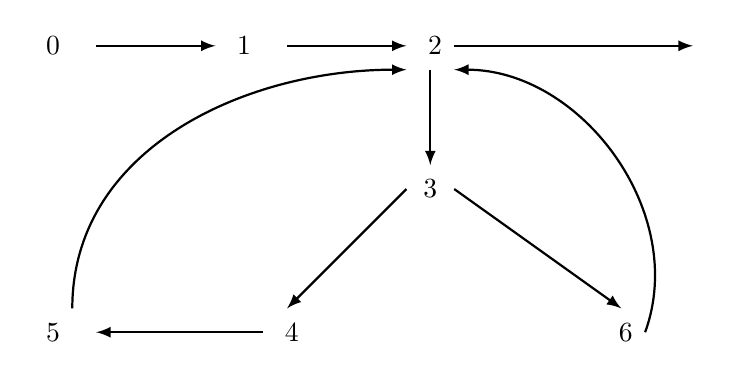
\begin{tikzpicture}[scale=\textwidth/20cm,samples=200]
  \draw[] (-8, 10) circle (0pt) node{{ $0$}};
  \draw[] (-4, 10) circle (0pt) node{{ $1$}};
  \draw[] (0, 10) circle (0pt) node{{ $2$}};
  \draw[] (0, 7) circle (0pt) node{{$3$}};
  \draw[] (-3, 4) circle (0pt) node{{ $4$}};
  \draw[] (-8, 4) circle (0pt) node{{ $5$}};
  \draw[] (4, 4) circle (0pt) node{{ $6$}};
  % Counter Variables
  \draw[] (6, 10) circle (0pt) node {\textbf{$\lex$}};
  % \draw[] (6, 4) circle (0pt) node {{ $ex$}};
  %
  % Control Flow Edges:
  \draw[ thick, -latex] (-7, 10)  -- (-4.5, 10);
  \draw[ thick, -latex] (-3, 10)  -- (-0.5, 10);
  \draw[ thick, -latex] (0, 9.5)  --  (0, 7.5) ;
  \draw[ thick, -latex] (0.5, 7)  --  (4, 4.5);
  \draw[ thick, -latex] (-7.5, 4.5)  to  [out=90,in=180]  (-0.5, 9.5);
  \draw[ thick, -latex] (4.5, 4)  to  [out=70,in=0] (0.5, 9.5);
  \draw[ thick, -latex]  (-0.5, 7) --   (-3, 4.5) ;
  \draw[ thick, -latex]  (-3.5, 4) --   (-7, 4) ;
  \draw[ thick, -latex] (0.5, 10)  --  (5.5, 10);
  % \draw[ thick, -latex] (6, 6.5)  -- node [right] {$\top$} (6, 4.5) ;
  \end{tikzpicture}
  \caption{}
    \end{centering}
    \end{subfigure}
  \caption{
  (a) The Two Paths While Loop Example
    (b) The Standard Execution Control Flow Graph}
      \label{fig:twoCountersWhile}
  \end{figure}
  }
\end{example}
\begin{enumerate}
  % \item  \textbf{The Abstract Execution Control Flow Graph} is generated in Figure~\ref{fig:threeNestedWhile}(b).
  \item \textbf{Rewrite The Program into The Language Model in~\cite{GulwaniJK09}}
  \[
    \begin{array}{l}
      \kw{twoPathsWhile}(k, m, N) \triangleq \\
      \rpasum(n > 0 \land m > 0);
      \clabel{ \assign{i}{n} }^{0} ; 
      \clabel{ \assign{j}{0} }^{1} ; \\
      \rprepeat(\rpasum(\clabel{i > 0}^{2}); \\
      \qquad \qquad \rpchoose\Big\{ 
        (\rpasum(\clabel{j < m}^{3}); \clabel{\assign{j}{j + 1}}^{4}; 
      \clabel{\assign{i}{i - 1}}^{5}),\\
      \qquad \qquad \qquad \qquad(\rpasum(\clabel{j \geq m}^{3}); \clabel{\assign{j}{0}}^{6})\Big\}
      );\\
      \rpasum(\clabel{i \leq 0}^{1})
      \end{array}
    \]

  \item \textbf{Program Refinement}
  \\
  % The loop free transition paths are computed as follows,
  \[
    \begin{array}{l}
      \kw{twoPathsWhile}(k, m, N) \triangleq \\
      \clabel{ \assign{i}{n} }^{0} ; 
      \clabel{ \assign{j}{0} }^{1} ; \\
      \rpchoose\Big\{ 
        \rprepeat(\rprepeat(\rpasum(\clabel{i > 0}^{2} \land \clabel{j < m}^{3}); \clabel{\assign{j}{j + 1}}^{4}; \clabel{\assign{i}{i - 1}}^{5});\\
      \qquad \qquad \qquad \qquad \rpasum(\clabel{i > 0}^{2} \land \clabel{j \geq m}^{3}); \clabel{\assign{j}{0}}^{6}),
      \\ \qquad \qquad 
      \rprepeat(\rpasum(\clabel{i > 0}^{2} \land \clabel{j < m}^{3}); \clabel{\assign{j}{j + 1}}^{4}; \clabel{\assign{i}{i - 1}}^{5}),\\
      \\ \qquad \qquad  \eskip
      \Big\};\\
      \rpasum(\clabel{i \leq 0}^{1})
      \end{array}
    \]
  % \[
  % \tpath_0 ; L_1: \rprepeat(\tpath_1; LOOP2: \rprepeat(\tpath_2; LOOP3 : \rprepeat(\tpath_3); \tpath_4); \tpath_5); \tpath_6
  % \]
Let $\rho_1 = \rpasum(\clabel{i > 0}^{2} \land \clabel{j < m}^{3}); \clabel{\assign{j}{j + 1}}^{4}; \clabel{\assign{i}{i - 1}}^{5}$
\\
and $\rho_2 = \rpasum(\clabel{i > 0}^{2} \land \clabel{j \geq m}^{3}); \clabel{\assign{j}{0}}^{6}$
  \item \textbf{Bound Computation}:
  \\
  % $L_1$, $L_2$ and 
  Let the $L$ denote the while loop at location $2$.
  % , $3$ and $6$ respectively.
  \\
  Step-by-Step of the BOUND computation in Figure~5 in \cite{GulwaniJK09}.
  \\
  \newcommand{\BD}{\mathcal{B}}
  $\BD(\kw{twoPathsWhile})$:
  \[
    \begin{array}{l}
      \BD(\kw{twoPathsWhile})  \triangleq  
      (c' + \max\{c'', c_1, c_2\} + c''', \emptyset \cup Z_1 \cup Z_2) 
      \\ \qquad
  \textbf{where} ~(c', \emptyset) \triangleq  \BD(\clabel{ \assign{i}{n} }^{0} ; \clabel{ \assign{j}{0} }^{1})
  \\ \qquad
  \textbf{and} ~(c'', \emptyset) \triangleq  \BD(\eskip)
  \\ \qquad
  \textbf{and} ~(c''', \emptyset) \triangleq  \BD( \rpasum(\clabel{i \leq 0}^{1}))
  \\ \qquad
  \textbf{and} ~(c_1, Z_1) \triangleq 
   \BD(L:  \rprepeat(\rprepeat(\rho_1); \rho_2))
      \\ \qquad
  \textbf{and} ~(c_2, Z_2) \triangleq  \BD(L: \rprepeat(\rho_1))
  %     \\ \qquad
  % \textbf{and} ~(c_3, Z_3) \triangleq  \BD(\rpasum(\clabel{i \geq k}^{1})) 
      \\ \qquad = (4, \{(2, L), (3, L)\})
    \end{array}
\]
\[
\begin{array}{l}
  \BD(L:  \rprepeat(\rprepeat(\rho_1); \rho_2)) \triangleq (0, Z \cup (c, L)) \\ \qquad
  \textbf{where} ~ c = c' + \sum\limits_{(c'', L'') \in Z' \land L = Parent(L'')}
  % \text{Definition}
  \\ \qquad
  \textbf{and} ~
  Z = \{(c'', L'') | (c'', L'') \in Z' \land L \neq Parent(L'')\}
  \\
  \qquad
  \textbf{and} ~ (c', Z') = \BD(\rprepeat(\rho_1); \rho_2))
  \\ \qquad = (0, \{(2, L), (3, L)\})
\end{array}
\]
\[
\begin{array}{l}
  \BD(\rprepeat(\rho_1); \rho_2))  \triangleq (c + 2, Z \cup \emptyset) 
  \\ \qquad
  \textbf{where} ~ (c, Z) \land \BD(L : \rprepeat(\rho_1))
  \\ \qquad = (2, \{( 3, L)\})
\end{array}
\]
\[
\begin{array}{l}
  \BD(L : \rprepeat(\rho_1))  \triangleq (0, Z \cup (c, L)) 
  \\ \qquad
  \textbf{where} ~ c = c' + \sum\limits_{(c'', L'') \in Z' \land L = Parent(L'')}
  % \text{Definition}
  \\ \qquad
  \textbf{and} ~
  Z = \{(c'', L'') | (c'', L'') \in Z' \land L \neq Parent(L'')\}
  \\
  \qquad
  \textbf{and} ~ (c', Z') = \BD(\rho_1)
  \\ \qquad = (0, \{(3, L)\})
\end{array}
\]
\[
\begin{array}{l}
  \BD(\rho_1)  \triangleq (3, \emptyset) 
\end{array}
\]
BOUND($\kw{twoPathsWhile}$):
\[
\begin{array}{l}
  BOUND(\kw{twoPathsWhile})
  \triangleq c + \sum\limits_{(c', L) \in Z}(c' \times T(L)) \textbf{where} ~ (c, Z) = (4, \{(2, L), (3, L)\})
  \\ \qquad 
  = 4 + 2 \times T(L) + 3 * T(L)
  \\ \qquad
  T(L) = \lfloor \frac{n}{m} \rfloor + m \times \lfloor \frac{n}{m} \rfloor
  %  \land c' = 5 + (6 + 2 \times N) \times m
  % \\ \qquad = 3 + 5 \times n + 6 \times m \times n + 2 \times m \times n \times N
\end{array}
\]
This step calls the perfect external
\\
$BOUNDFINDERD(INIT(L, 0, 2), NEXT(L, 0, 2), \{m, n\})$.
It computes $T(L)$, which is the number of iterations for the while loop at location $1$.
We assume that it perfectly computes the $T(L) = \lfloor \frac{n}{m} \rfloor + m \times \lfloor \frac{n}{m} \rfloor$.
\end{enumerate}